\documentclass{beamer}

%%% -------------- CREATE HANDOUTS -----------------------------------
%\documentclass[12pt, handout]{beamer}
%\usepackage{pgfpages}
%\pgfpagesuselayout{4 on 1}[letterpaper, landscape, border shrink=5mm]
%%% ------------------------------------------------------------------


\mode<presentation>
  \usepackage{ru}
  %\usetheme{Warsaw}
  %\usecolortheme{seahorse}
  %\usefonttheme{default}
  \setbeamertemplate{caption}[numbered]
  %\setbeamertemplate{headline}{}
  %\setbeamertemplate{navigation symbols}{}
  \setbeamertemplate{bibliography item}[text]
\newcommand*\oldmacro{}%
	\let\oldmacro\insertshorttitle%
%\renewcommand*\insertshorttitle{%
%   \oldmacro\hfill%
%   \insertframenumber\,/\,\inserttotalframenumber}
\setbeamertemplate{section page}{
    \begin{centering}
    \vspace{1cm}
    \begin{beamercolorbox}[rounded=true,shadow=false,sep=4pt,center]{part title}
    \usebeamerfont{section title}\LARGE{\insertsection}\par
    \end{beamercolorbox}
    \end{centering}}
\usepackage{ragged2e}
\usepackage[english]{babel}
\usepackage[utf8]{inputenc}
\usepackage{appendixnumberbeamer}
\usepackage{natbib}
\usepackage{textpos}
\usepackage{lipsum}
\usepackage{tikz}
\usepackage[percent]{overpic}
\usepackage{textcomp}
\usepackage{booktabs}
\usepackage{mathabx}
\usepackage{pifont}
\usepackage{bbding}
\usepackage{fontenc}
%\let\Sun\undefined   %to undefine something
%\usepackage{marvosym}
%\usepackage{scalerel}
%% \usepackage[
%%   style=numeric,
%%   citestyle=authoryeartitle
%% ]{biblatex}
\setbeamerfont{caption}{size=\tiny}

%\setbeameroption{show notes}
%\setbeamertemplate{note page}[plain]
\newcommand{\tss}{\textsuperscript}
\newcommand{\tsbs}{\textsubscript}
%Change Bullets in latex list
\setbeamertemplate{itemize item}{\scriptsize\raise1.25pt\hbox{\donotcoloroutermaths\ding{118}}}
\setbeamertemplate{itemize subitem}{\scriptsize\raise1.25pt\hbox{\ding{226}}}
\setbeamertemplate{itemize subsubitem}{\tiny\raise1.25pt\hbox{\ding{169}}}
\setbeamertemplate{enumerate item}{\insertenumlabel.}





%% \title{The Title}
%% \subtitle{The Subtitle}
%% \author{The Author}
%% \supervisor{David Hilbert}
%% \institute{The Institute}



%%To select specific font
%{\fontsize{2.5}{4}\selectfont tobesize}

%\setbeamertemplate{background}{\tikz[overlay, remember picture]\node[xshift=-2.3cm, yshift=1.50cm, opacity=0.4]at (current page.south east){
\includegraphics[width=4cm]{images}};}

%\title[Decontamination Factors for Nuclear Forensics]{Experimental Characterization of Pu Separation by %PUREX Process on a Low-Burnup, Pseudo-Fast-Neutron Irradiated DUO\tsbs{2} for Product Decontamination Fa%ctors and Nuclear Forensics}
%\author{Paul Mendoza}
%

\title[Your Short Title]{Your Presentation}
\institute{Where You're From}
\author{
        Author:       Me \\[1ex]
        Supervisors:  First                  Second
}
\date{02/27/2017}

\begin{document}

\setbeamertemplate{caption}{\raggedright\insertcaption\par}
\begin{frame}
	%% background
  \tikz[overlay, remember picture]\node[xshift=-3.5cm, yshift=3cm, opacity=0.1]at (current page.south east){
\includegraphics[width=8cm]{tamu_system_proposed_seal_042915}};
	%% Left-hand logo
  \begin{tikzpicture}[remember picture, overlay]
  \node [xshift = 3 cm, yshift=1.2cm] at (current page.south west){
\includegraphics[width=5cm]{tees_logo_primary_maroon}};
  \end{tikzpicture}
    %% Right-hand logo
  \begin{tikzpicture}[remember picture, overlay]
  \node [xshift = -3cm, yshift=1.2cm] at (current page.south east){
\includegraphics[width=5cm]{TEES_NSSPI_logo_HMaroon}};
  \end{tikzpicture}
  %% Upper logo right
    \begin{tikzpicture}[remember picture,overlay]
    \node[anchor=north east,yshift=2pt] at (current page.north east) {
\includegraphics[height=0.8cm]{NUENlogo}};
    \end{tikzpicture}
  %% Upper logo left
    %% \begin{tikzpicture}[remember picture,overlay]
    %% \node[anchor=north west,yshift=2pt] at (current page.north west) {
\includegraphics[height=0.8cm]{NUENlogo}};
    %% \end{tikzpicture}
    \titlepage
    \vspace{-1.8cm}
    \begin{center}
      Presented at All Hands Meeting
    \end{center}
\end{frame}

%Add Biola Seal
\setbeamertemplate{background}{\tikz[overlay, remember picture]\node[xshift=-2.5cm, yshift=2.5cm, opacity=0.05]at (current page.south east){
\includegraphics[width=6cm]{imageedit_2_7317234434}};}

%Add NSSPI to upper right
\addtobeamertemplate{frametitle}{}{%
  \begin{tikzpicture}[remember picture,overlay]
    \node[anchor=north east,yshift=2pt] at (current page.north east) {
\includegraphics[height=0.8cm]{NUENlogo}};
  \end{tikzpicture}
    \begin{tikzpicture}[remember picture,overlay]
      \node[anchor=north west,yshift=2pt] at (current page.north west) {
\includegraphics[height=0.8cm]{TEES_NSSPI_Acronym_logo_WHT}};
  \end{tikzpicture}
}


\begin{frame}{Outline}
\tableofcontents
\end{frame}

\section{Motivation}
\begin{frame}{Big Picture}
  %\vspace{-1cm}
  \begin{itemize}
  \item{Weapons-grade Pu can be extracted from reactor discharged fuel
    with a burnup of about 1 (GWD/tU)}
  \item{Pu isotopes produced in irradiated fuel can vary} %depending on}
    %% \begin{itemize}
    %% \item{Burnup (irradiation history)}
    %% \item{Reactor neutron spectrum (core design)}
    %% \end{itemize}
  \item{Two examples of reactors which can intentionally
  discharge low burned fuel for extracting weapon-grade Pu are:}
  \begin{itemize}
  \item{Fast Breeder Reactor}
    \note[item]{Madras Atomic Power Station Kalpakkam, India}
    \note[item]{Expected criticality in Jan 2017}
    \note[item]{Cost from 450 million euros to 750 euros}
    \note[item]{Sodium-cooled reactor design - U238 for breeding}
    \note[item]{100 GWd/t for core, 40 year life, 1750 tonnes of sodium
      about 75\% of olympic sized swimming pool.}
    \note[item]{liquid sodium has a density a little less than water}
    \note[item]{MOX fuel (UO2 and PuO2) fuel}
    \note[item]{Fuel discharged at 100GWd/t, but I just mentioned
      that we are worried about 1GWd/t, mistake?}
  \item{CANDU Reactor
          \begin{figure}[H]
        \begin{flushright}
	   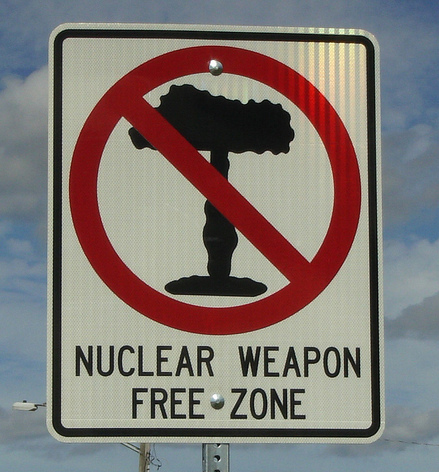
\includegraphics[scale = 0.2]{nuclear-weapons-free-zone}
	\end{flushright}
      \end{figure}}
  \end{itemize}
%\item{In accord with the Indo-US 123 agreement, these reactors were not
%      required to be kept under IAEA safeguards}
  \end{itemize}
  %% \begin{tikzpicture}[remember picture, overlay]
  %%   \node [xshift = -3cm, yshift=1.2cm] at (current page.south east){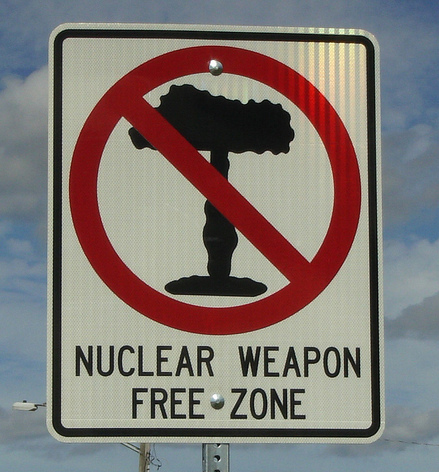
\includegraphics[width=5cm]{nuclear-weapons-free-zone}};
  %% \end{tikzpicture}
\end{frame}

\begin{frame}{Smaller Picture}
  \begin{columns}
    \begin{column}{0.5\textwidth}
      \vspace{-10mm}
      \begin{itemize}
      \item{Attribution for unpurified Pu has been previously studied
        \tss{\cite{chirayath2015trace,scott2005nuclear,glaser2009isotopic}}}
      \item{Interdicted Pu would likely have been processed}
      \item{Lack of literature on decontamination factors and
        distribution coefficients for useful forensic elements (Cs, Sb,
        Eu, Rb, Sr, Nd, Pm, and Sm)} 
      \end{itemize}
    \end{column}
    \begin{column}{0.5\textwidth}
      \begin{figure}[H]
        \vspace*{-1cm}
        \begin{center}
	  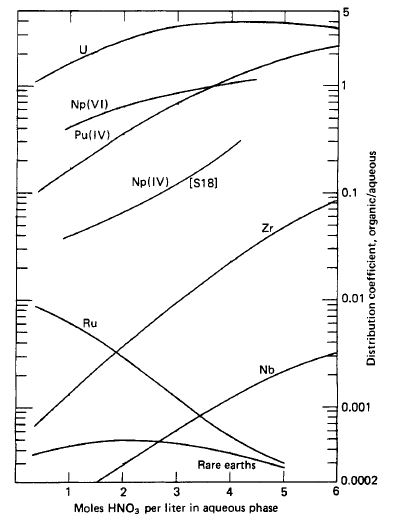
\includegraphics[scale = 0.5]{Stoller}
          \vspace{-0.5cm}
           \caption{\tiny{Adapted from Stoller\tss{\cite{stoller1961reactor}}}}
	\end{center}
      \end{figure}
    \end{column}
  \end{columns}  
\end{frame}


\section{Background}
\begin{frame}
\sectionpage
\end{frame}

\subsection{The PUREX Process}
\begin{frame}{What is PUREX - A type of laundry detergent?}
  \vspace{0.5cm}
  \begin{itemize}
  \item Plutonium Uranium Redox EXtraction 
    \begin{itemize}
    \item Liquid-liquid solvent extraction
    \item Many stages:
      \begin{enumerate}
      \item{Preparation for Dissolution}
      \item{Dissolution}
      \item{Preparation of Dissolved Feed}
      \item{Primary Decontamination - Extraction to
        organic\textsuperscript{\tiny{\AsteriskThin}}}
      \item{Scrubbing}
      \item{Plutonium Partition - Back-Extraction to
        aqueous\textsuperscript{\tiny{\AsteriskThin}}}
      \item{Plutonium Purification}
      \end{enumerate}
    \end{itemize}
  \end{itemize}
  \vspace{1.5cm}
  \textsuperscript{\tiny{\AsteriskThin\hspace{1mm}- Discussing Next}}
\end{frame}


\begin{frame}{Extraction}
  $UO_{2(aq)}^{2+}+2NO^{-}_{3(aq)}+2TBP_{(o)}
  \leftrightarrow UO_2(NO_3)_2\cdot2TBP_{(o)}$\tss{\cite{benedict1982nuclear}}
  $Pu^{4+}_{(aq)}+4NO^{-}_{3(aq)}+2TBP_{(o)}
  \leftrightarrow Pu(NO_3)_4\cdot 2TBP_{(o)}$
  \note[item]{Most of the fission products are
    left in the aqueous solution
    at valence III and V states\tss{\cite{kok2009nuclear}}}
  \vspace{-3mm}
  \begin{figure}[H]
    \vspace*{0.1cm}
    \begin{center}
      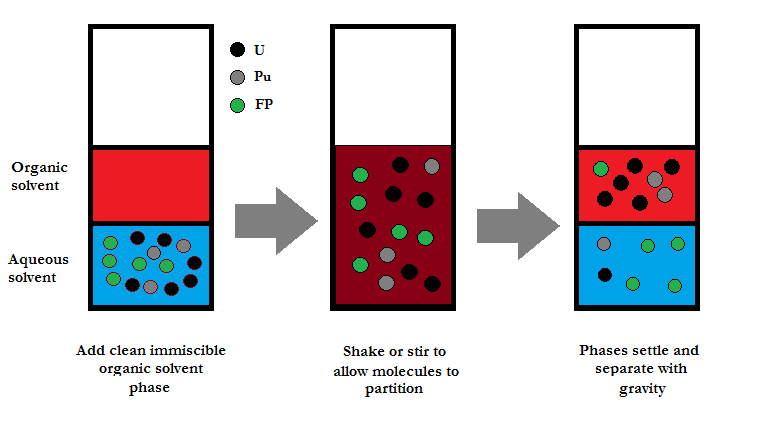
\includegraphics[scale = 0.5]{Extraction}
    \end{center}
  \end{figure}
\end{frame}

\begin{frame}{Back-Extraction}
  $Pu(NO_3)_4(TBP)_{2(o)}+Fe^{2+}_{(aq)}\leftrightarrow Pu^{3+}_{(aq)}+4NO^{-}_{3(aq)}+2TBP_{(o)}$\tss{\cite{konings2006chemistry}}
  \note[item]{The fission products that contribute mostly
    to the radioactive contamination of product in PUREX
    are zirconium, niobium, and ruthenium - with multiple
    oxidation states.}
  \begin{figure}[H]
    \vspace*{0.1cm}
    \begin{center}
      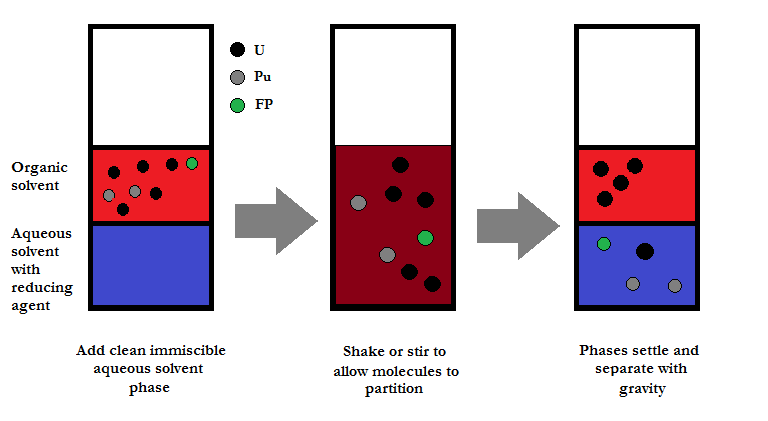
\includegraphics[scale = 0.5]{Back_Extraction}
    \end{center}
  \end{figure}
\end{frame}


%% \begin{frame}{Extraction and Back-extraction}
%%   \begin{columns}
%%     \begin{column}{0.5\textwidth}
%%       \vspace{-3mm}
%%       \begin{itemize}
%%       \item{Extraction}

%%       \item{Back-extraction}
%%         \begin{itemize}
%%           \item{An item}

%%         \end{itemize}
%%       \end{itemize}
%%     \end{column}
%%     \begin{column}{0.5\textwidth}

%%     \end{column}
%%   \end{columns}  
%% \end{frame}

\subsection{Distribution Coefficients}
\begin{frame}{Distribution Coefficients - The Missing link}
  \begin{itemize}
  \item{Distribution Coefficient (D): The ratio between the organic
  and aqueous phases (aka: D-values)}
    \begin{equation*}
      D=\frac{c_{o}}{c_{aq}}
    \end{equation*}
    \note[item]{Distribution coefficients can be reported
      in terms of volume basis (weight per unit volume), or a
      mass basis (mass of solute per unit mass of solute free
      solvent)- usually reported on volume basis}
  \item{Specific element to element}
  \item{Vary widely with:\tss{\cite{stoller1961reactor}}}
    \begin{itemize}
    \item{Composition of phases}
    \item{Solution saturation}
    \item{Temperature of the solvent}
    \end{itemize}
  \item{The fraction of mass, $f_o$ deposited in the organic
    phase, assuming a volume ratio between
    the aqueous and organic phases, $V_R$, is:}
    \begin{equation*}
      f_o=(1+D^{-1}V^{-1}_R)^{-1}
    \end{equation*}
    \note[item]{Note not a function of density, even though
      the two solutions have different densities, when solving for
      this value it cancels out}
    \note[item]{Solved this way to show, volume matters, and to give
      me a more intuitive sense of where things are going}
  \end{itemize}
\end{frame}

\subsection{Decontamination Factors}
\begin{frame}{Decontamination Factors - The Pot of gold}
  \begin{itemize}
  \item{After several cycles of Pu extraction/scrubbing/back-extraction
    are completed, the effectiveness of a PUREX cycle is described
    by the decontamination factor (DF):}
    \begin{equation*}
      DF_j=\frac{\left|\frac{c_j}{c_{Pu}}\right|_{initial}}
      {\left|\frac{c_j}{c_{Pu}}\right|_{final}}
    \end{equation*}
  \item{DFs are characteristic of different process cycles}
  \item{Larger values (10\tss{7}) for industrial scale PUREX (compared
  to benchtop)\tss{\cite{stoller1961reactor,benedict1982nuclear}}}
  \end{itemize}
\end{frame}

%% \begin{frame}{Complexity of reprocessing schemes}
%%   \begin{figure}[H]
%%     \vspace*{-1cm}
%%     \begin{center}
%%       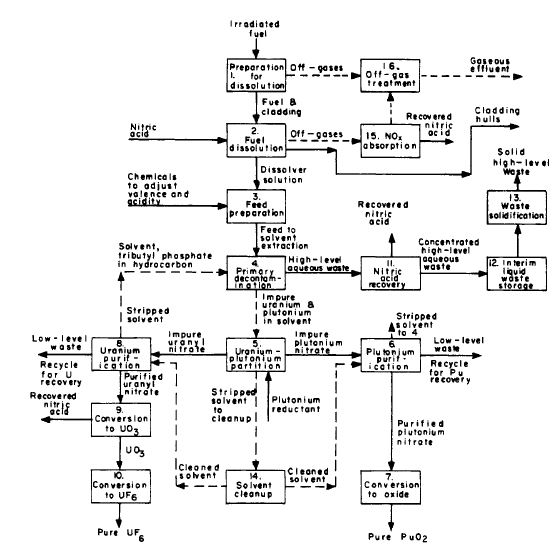
\includegraphics[scale = 0.4]{PUREX_Process}
%%       \caption{\tiny{Principal steps in PUREX\tss{\cite{benedict1982nuclear}}}}
%%     \end{center}
%%   \end{figure}
%%   \note[item]{Worry about dependancies of of DC
%%   Worry about non equilibrium
%%   flow rates, blah blah blah.
%%   Show mixer settler columns, show batch.
%%   What I want to do, get some distribution coefficients
%%   develop a reasonable process for isolating a large
%%   fraction of Pu, then, based on process, calculate what
%%   the decontamination factor should be, and then actually measure it}
%% \end{frame}


%% \begin{frame}{Complexity of reprocessing schemes}
%%   \begin{figure}[H]
%%     \vspace*{-1cm}
%%     \begin{center}
%%       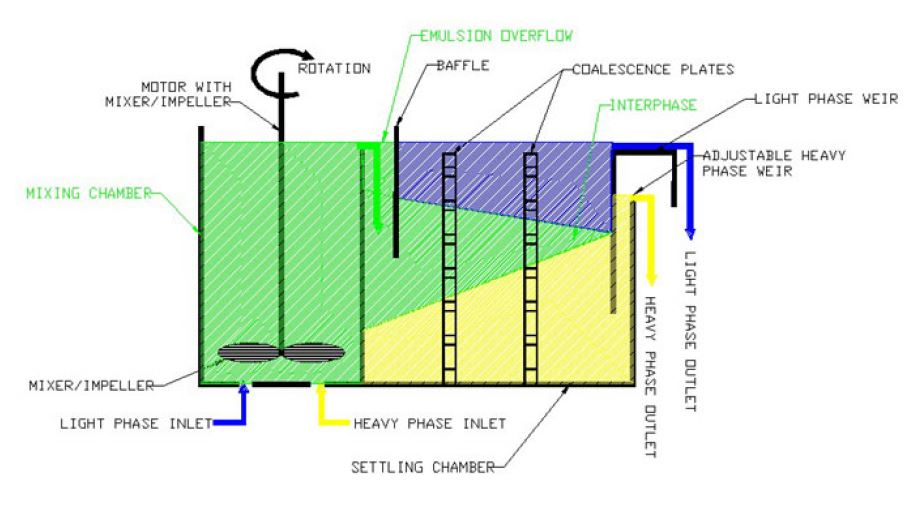
\includegraphics[scale = 0.4]{mixer}
%%       \caption{\tiny{Mixer-Settler Diagram}}
%%     \end{center}
%%   \end{figure}
%% \end{frame}


%% \begin{frame}{Complexity of reprocessing schemes}
%%   \begin{figure}[H]
%%     \vspace*{-1cm}
%%     \begin{center}
%%       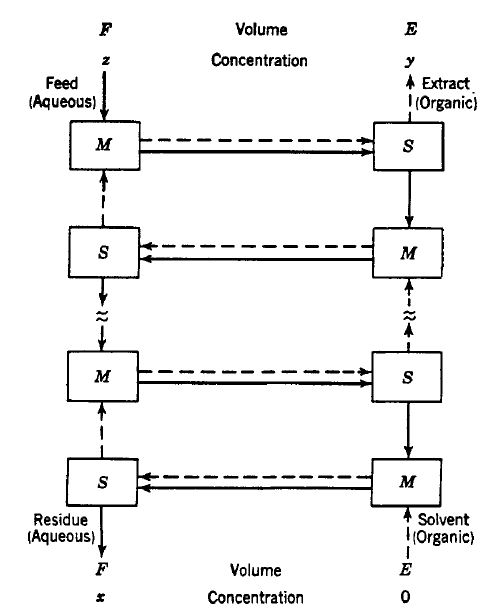
\includegraphics[scale = 0.35]{stage}
%%       \caption{\tiny{Multistage countercurrent solvent extraction.
%%           M, mixer; S, settler.\tss{\cite{benedict1982nuclear}}}}
%%     \end{center}
%%   \end{figure}
%% \end{frame}


%% \begin{frame}{Complexity of reprocessing schemes}
%%   \begin{figure}[H]
%%     \vspace*{-1cm}
%%     \begin{center}
%%       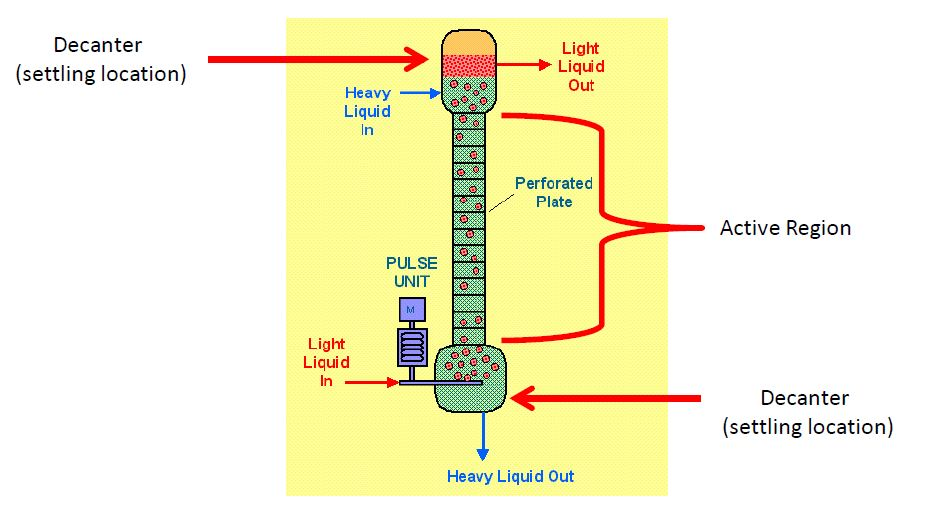
\includegraphics[scale = 0.4]{column}
%%       \caption{\tiny{Pulsed Column Diagram}}
%%     \end{center}
%%   \end{figure}
%% \end{frame}

\section{Previous Work}
\begin{frame}
\sectionpage
\end{frame}

\subsection{Experiment}
\begin{frame}{Irradiation}
  \begin{columns}
    \begin{column}{0.5\textwidth}
      \vspace{-1cm}
      \begin{itemize}
      \item{12.9 $\pm$ 0.1 mg of DUO\tsbs{2} was irradiated}
        \begin{itemize}
        \item{High Flux Isotope Reactor at Oak Ridge National Laboratory}
        \end{itemize}
      \item{Burnup was 4.43 $\pm$ 0.31 GWd/tHM\tss{\cite{swinney2015experimental}}}
      \item{0.196 $\pm$ mg of total Pu was produced as measured by ICP-MS}
      \end{itemize}
    \end{column}
    \begin{column}{0.5\textwidth}
      \begin{figure}[H]
        \vspace*{-1cm}
        \begin{center}
	   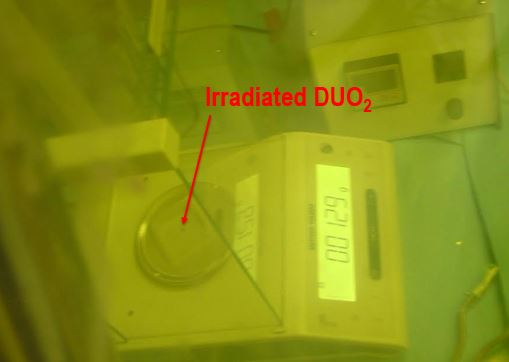
\includegraphics[scale = 0.4]{irradiated}
           %\caption{\tiny{Picture of irradiated sample}}
	\end{center}
      \end{figure}
    \end{column}
  \end{columns}  
  \end{frame}

\begin{frame}{Dissolution of the spent fuel pellet}
      \begin{figure}[H]
        \vspace*{-1cm}
        \begin{center}
	   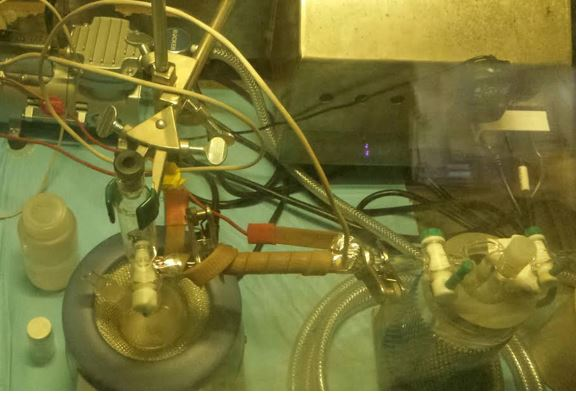
\includegraphics[scale = 0.65]{dissolution}
	\end{center}
      \end{figure}
\end{frame}

\begin{frame}{Glovebox}
      \begin{figure}[H]
        \vspace*{-1cm}
        \begin{center}
	   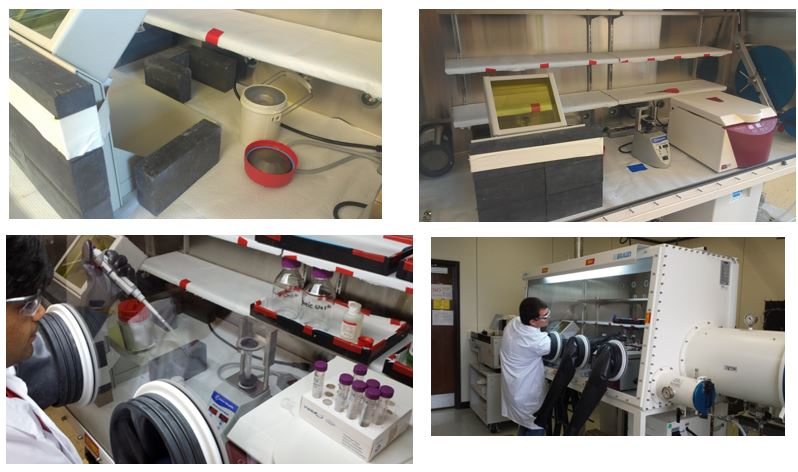
\includegraphics[scale = 0.5]{glovebox}
	\end{center}
      \end{figure}
\end{frame}

\begin{frame}{Experiments}
  \begin{itemize}
  \item{Single stage extraction and back-extraction}
    \begin{itemize}
    \item{Purpose: quantify product recovery, D-values and DF values
      for single stage extraction and back extraction}
    \item{Conditions:}
    \end{itemize}
  \end{itemize}
  \begin{center}
    \vskip -0.2cm
    {\fontsize{2.5}{4}\selectfont
      \begin{tabular}{l  c  c}\toprule
        Starting Solution  & Extraction Solution
        & Back extraction solution \\ \midrule \vspace{0.1cm}
        4 M nitric acid & 30\% vol.\% TBP, 70 vol.\% kerosene & 0.024 M ferrous sulfamate in 0.75 M nitric acid \\ \bottomrule
      \end{tabular}
      }
  \end{center}
  \begin{itemize}
  \item{Multi-contact extraction and back-extraction}
    \begin{itemize}
    \item{Purpose: Maximize recovery of Pu with 4 extractions,
      3 back extractions}
    \item{Conditions:}
    \end{itemize}
  \end{itemize}
    \begin{center}
    \vskip -0.2cm
    {\fontsize{2.5}{4}\selectfont
      \begin{tabular}{l  c  c}\toprule
        Starting Solution  & Extraction Solution
        & Back extraction solution \\ \midrule \vspace{0.1cm}
        4 M nitric acid & 30\% vol.\% TBP, 70 vol.\% kerosene & 0.024 M ferrous sulfamate in 4 M nitric acid \\ \bottomrule
      \end{tabular}
      }
  \end{center}
\end{frame}

\subsection{Recovery of Pu and U}
\begin{frame}{Previous Experiment Results}
  \begin{block}{Recoveries of U and Pu}
    \begin{center}
      \vskip -0.2cm
   %{\fontsize{2.5}{4}\selectfont
  \begin{tabular}{l  c  c}\toprule
                & Pu Recovery & U Recovery \\ \midrule \vspace{0.1cm}
   Single stage         & (83.4$\pm$9.5)\% & (11.2$\pm$1.3)\% \\
   Multi-contact Cycle 1 & (99.7$\pm$4.2)\% & (6.8$\pm$0.3)\% \\
   Multi-contact Cycle 2 & (93.0$\pm$4.6)\% & (6.6$\pm$0.3)\% \\
   Overall Experiment 2 & (92.7$\pm$6.0)\% & (0.45$\pm$0.03)\% \\ \bottomrule
  \end{tabular}
  %}
  \end{center}
  \end{block}
\end{frame}

\subsection{Experimental Decontamination Factors}
\begin{frame}{Previous Experiment Results}
  \vspace{-0.6cm}
  \begin{block}{Decontamination Factors}
    \begin{center}
      \vskip -0.2cm
  {\fontsize{7}{11.2}\selectfont
  \begin{tabular}{l  c  c c c c}\toprule
   Element (Z)  & SS & Error & MC Cycle 1 & Error & Isotopes Used\\ \midrule 
   Rb(37) & 39.0 & 5.9 & 11.8 & 0.8 & $^{85}$Rb \\
   Sr(38) & 283  & 43  & 84.6 & 5.9 & $^{90}$Sr \\
   Mo(42) & 5.7  & 0.8 & 1.9  & 0.2 & $^{97,98,100}$Mo \\
   Ru(44) & 59.2 & 6.4 & 16.6 & 2.5 & $^{101,102,104}$Ru \\
   Pd(46) & 65   & 14  & 8.9  & 1.2 & $^{110}$Pd \\
   Cd(48) & 74   & 17  & 22.1 & 2.5 & $^{112}$Cd \\
   Cs(55) & 177  & 28  & 52.9 & 3.9 & $^{133}$Cs \\
   Ce(58) & 43   & 16  & 11.5 & 4.9 & $^{140,142}$Ce \\
   Nd(60) & 19.2 & 2.1 & 5.9  & 0.4 & $^{143}$Nd \\
   Pm(61) & 12.8 & 1.9 & 3.9  & 0.3 & $^{147}$Pm \\
   Sm(62) & 11.5 & 1.5 & 3.6  & 0.3 & $^{151}$Sm \\
   Eu(63) & 10.0 & 1.4 & 3.6  & 0.3 & $^{154}$Eu \\
   U(92) & 7.4   & 1.2 & 14.7 & 0.9 & $^{238}$U \\ \bottomrule
  \end{tabular}
  }
  \end{center}
  \end{block}
\end{frame}

\begin{frame}{Conclusions}
  \begin{itemize}
  \item{Two PUREX experiments were conducted}
    \begin{itemize}
    \item{Single stage: Determined DC values for Pu, U and several FP}
    \item{Multi-contact: Utilized Experiment 1 to recover over 92\%
      of Pu while leaving less than 1\% of the U}
    \end{itemize}
  \item{DF values were measured for 12 FP elements}
  \item{DF values were lower than those typically found in industrial
    scale PUREX plants due to multiple extraction and back-extraction
    steps without an intermittent scrubbing step.}
  \item{This work provide DF data that will be built upon for
        nuclear forensic investigations of interdicted Pu.}
  \end{itemize}
\end{frame}


\section{Future Work}
\begin{frame}
\sectionpage
\end{frame}

\begin{frame}{Future Work}
  \begin{itemize}
  \item{Modify Multi-contact extraction, to recover a larger
    fraction of Pu}
  \item{Investigation of how D-values for (Cs, Sb,
    Eu, Rb, Sr, Nd, Pm, and Sm) change as a function of
    nitric acid concentration}
  \item{Determine statistical uncertainty of D and DF values.}
    \begin{itemize}
    \item{Repeat above experiments 3-5 times}
    \end{itemize}
  \item{Connect D-values with process information to DF values}
\end{itemize}
\end{frame}

\appendix
\section{Questions?}
\begin{frame}
\sectionpage
\end{frame}

\begin{frame}{Previous Experiment Results}
  \begin{figure}[H]
    \vspace*{-.1cm}
    \begin{center}
      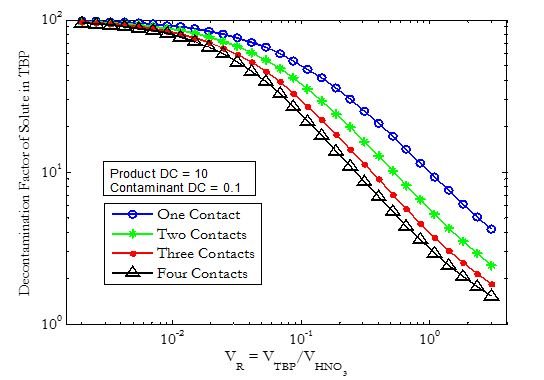
\includegraphics[scale = 0.6]{df}
      \vspace{-0.5cm}
      \caption{\tiny{Decontamination Factors for multi-contact extraction.}}
    \end{center}
  \end{figure}
\end{frame}

\begin{frame}[allowframebreaks]{References}
\def\newblock{}
\nocite{*}
\scriptsize{\bibliographystyle{plain}}
\bibliography{references}
\end{frame}

\begin{frame}{Mass Spec}
  \begin{figure}[H]
    \vspace*{-1cm}
    \begin{center}
      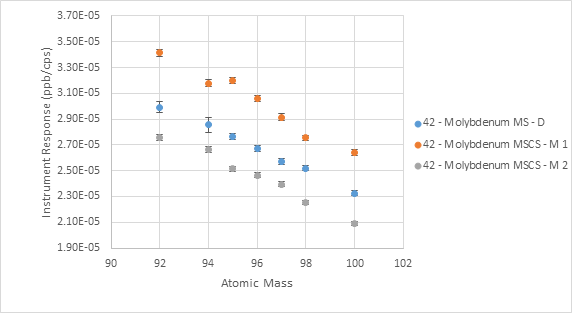
\includegraphics[scale = 0.75]{instrument_response}
    \end{center}
  \end{figure}
\end{frame}

\end{document}
